\documentclass[twocolumn,
			   showpacs,%
               nofootinbib,
               aps,%
               %eqsecnum,
               prd,
               notitlepage,
               showkeys,
               10pt]{revtex4-1}
               
%Loading my personal settings
\usepackage{todonotes}

%math and formulas
\usepackage{amssymb}
\usepackage{amsmath}
\usepackage{physics}

%language settings and microtype
\usepackage[english]{babel}
\usepackage{microtype}

%useful packages
\usepackage{graphicx}
\usepackage{siunitx}
\usepackage{xcolor}
\usepackage{float}
\usepackage{dcolumn}
\usepackage{blindtext}
\usepackage{xfrac}
\usepackage[labelfont=bf]{caption}
\usepackage{subcaption}


%feynman diagrams
\usepackage{tikz}
\usepackage{tikz-feynman}
\tikzfeynmanset{compat=1.0.0} 

%loading the `external` library
\usetikzlibrary{external}   
%Create directory to store the diagrams and all related files          
\immediate\write18{mkdir -p feynman-diagrams} 
% Activate externalization
\tikzexternalize[
  %Avoid cluttering the directory                     
  prefix=feynman-diagrams/, 
  %Calling lualatex externally
  system call={             
    lualatex \tikzexternalcheckshellescape -halt-on-error -interaction=batchmode -jobname="\image" "\texsource"  || rm "\image.pdf"
  },
]

%color settings
\definecolor{mydarkblue}{RGB}{1,1,141}

%correcting parindent
\setlength{\parindent}{0pt}


%always use hyperref at the end of the preamble!
\usepackage[colorlinks=True]{hyperref}
\hypersetup{allcolors=mydarkblue}
%main document
\begin{document}

%Personel data
\title{F91: Studying the $Z$ boson with the ATLAS Detector at the LHC }
\author{Mathieu Kaltschmidt}
\email{M.Kaltschmidt@stud.uni-heidelberg.de}
\affiliation{Heidelberg University,  D-69117 Heidelberg, Germany}
\author{Quirinus Schwarzenb\"ock}
\email{Schwarzenb\"ock@stud.uni-heidelberg.de}
\affiliation{Heidelberg University,  D-69117 Heidelberg, Germany}

\date[Carried out in the week of  ]{March 4$^{\text{th}}$, 2019}


\begin{abstract}
This experiment has been performed as part of the advanced lab course for physics students (FP) at Heidelberg University.
The goal of this computer-based experiment is to determine the invariant mass spectrum for the $Z$ boson, one of the three massive gauge bosons of the weak interaction, using data acquired by the ATLAS experiment at the Large Hadron Collider (LHC) at CERN in Geneva.  A multi-level filter system is implemented to get a clean mass distribution of the measured $Z$ boson candidates. For data-analysis  and plotting we use \verb|ROOT| and different \verb|Python3| scipts.
\end{abstract}

\maketitle



\section{Introduction}
Taking the geometric properties into account, it is very easy to see the following connection between momentum and transversal momentum
\begin{align}
	p_x &= p_T \cos(\phi)\\
	p_y &= p_T \sin(\phi)\\
	p_z \tan(\theta) &= p_T
\end{align}
From the definition of the pseudorapidity (eq: \ref{pseudorapidity}) we have $\theta = 2\arctan(e^{-\eta})$. Using the identity $\tan(2\arctan(x)) = \frac{2x}{1 - x^2}$, these equations lead to 
\begin{align}
	p_z &= p_T\sinh(\eta)\\
	\left|\mathbf{p}\right| &= p_T \cosh(\eta)
\end{align}



Already implementing the formulas mentioned in the theory part of \cite{F91manual} to speed things up a little.
\begin{align}
\mathcal{L} = \frac{N_1N_2f_{\text{rev}}n_b}{4\pi\sigma_x\sigma_y}
\end{align}

\blindtext

\begin{align}
\mathcal{L}_{\text{int}} = \int \mathcal{L} \ \dd t	
\end{align}

\blindtext

\begin{align}
N = \sigma_{pp\rightarrow X} \cdot \mathcal{L}_{\text{int}}
\end{align}


\section{Theory}


\begin{figure}[H]
\centering	
\feynmandiagram [small] [horizontal' = a to b] {
	i1 [particle=\(\overline{u}\)] -- [fermion] a  -- [fermion] i2 [particle=\(d\)],
	a -- [photon, edge label=\(W^{-}\)] b ,
	f1 [particle=\(\nu_{e^{-}}\)] -- [fermion] b -- [fermion] f2 [particle=\(e^{-}\)],
	};
\caption{1-Lepton final state.}
\end{figure}

\begin{figure}[H]
\centering	
\feynmandiagram [small] [horizontal' = a to b] {
	i1 [particle=\(q\)] -- [fermion] a  -- [fermion] i2 [particle=\(\overline{q}\)],
	a -- [photon, edge label=\(\gamma / Z^0\)] b ,
	f1 [particle=\(e^{+}\)] -- [fermion] b -- [fermion] f2 [particle=\(e^{-}\)],
	};
\caption{2-Lepton final state.}
\end{figure}

\begin{figure}[H]
\centering	
\begin{tikzpicture}
  \begin{feynman}
    \vertex (a) {\(d\)};
    \vertex [right=of a] (b);
    \vertex [above right=of b] (c);
    \vertex [above right=of c] (f1) {\(e^{-}\)};
    \vertex [below right=of c] (f2) {\(\overline{\nu}_{e^{-}}\)};
    \vertex [below =of a] (d) {\(\overline{u}\)};
    \vertex [right=of d] (e);
    \vertex [below right=of e] (f);
     \vertex [above right=of f] (f3) {\(e^{-}\)};
    \vertex [below right=of f] (f4) {\(e^{+}\)};

 
    \diagram* {
      (a) -- [fermion] (b) -- [boson, edge label=\(W^{-}\)] (c),
      (d) -- [anti fermion] (e) -- [boson, edge label'=\(Z^{0}\)] (f),
      (f1) -- [anti fermion] (c) -- [anti fermion] (f2),
      (f3) -- [anti fermion] (f) -- [anti fermion] (f4),
      
      (b) -- [edge label' = \(\overline{u}\) ] (e),
};
  \end{feynman}
\end{tikzpicture}
\caption{3-Lepton final state.}
\end{figure}


\section{Experiment}

\begin{figure}[H]
\centering
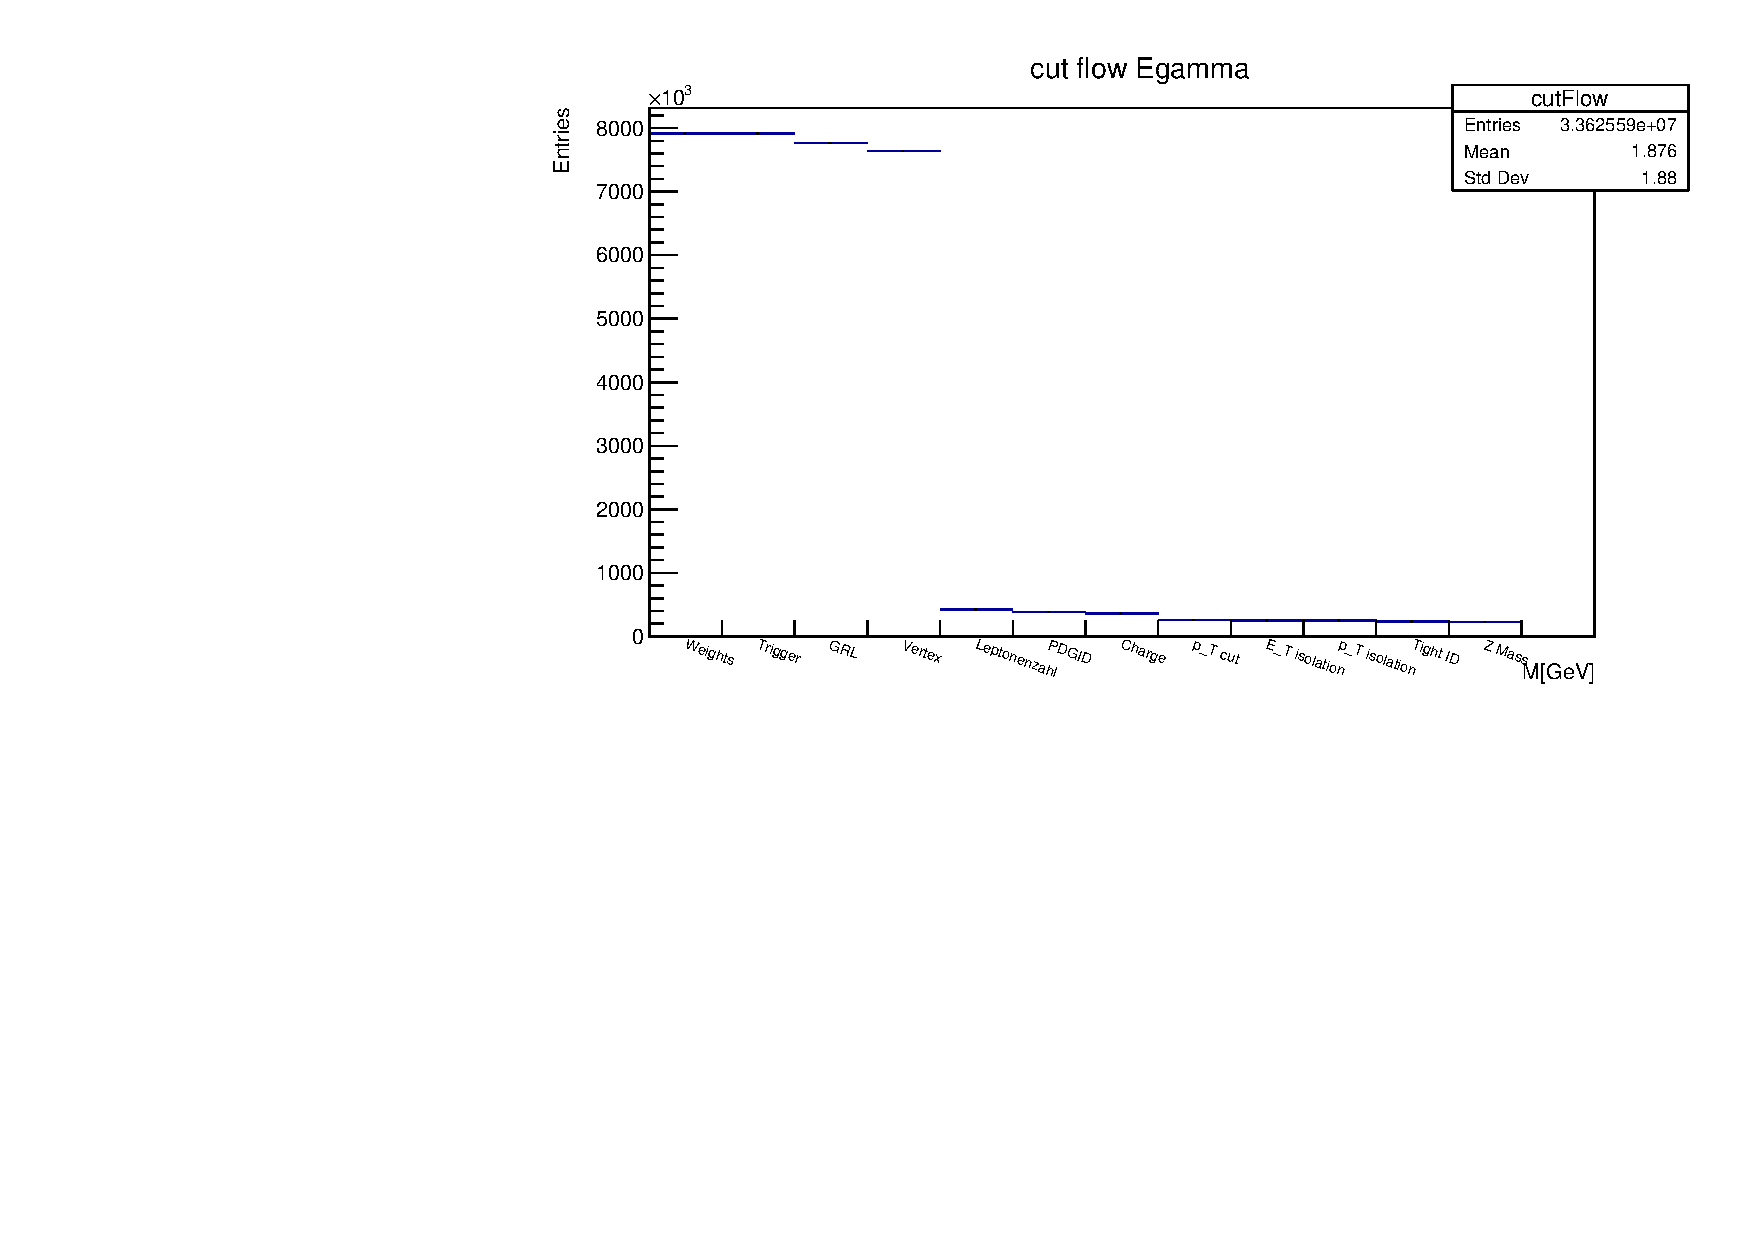
\includegraphics[width = 0.45\textwidth]
{figures/plots/CutFlow}
\caption{Cut flow diagram for our event selection algorithm.}	
\end{figure}



\section{Results}

We want to use this section to present the final result for the mass distribution of the processes with $Z$-candidates which passed all filter levels. The result is presented in the following in figure (\ref{fig:MassDist}).

\begin{figure}[H]
	\centering
	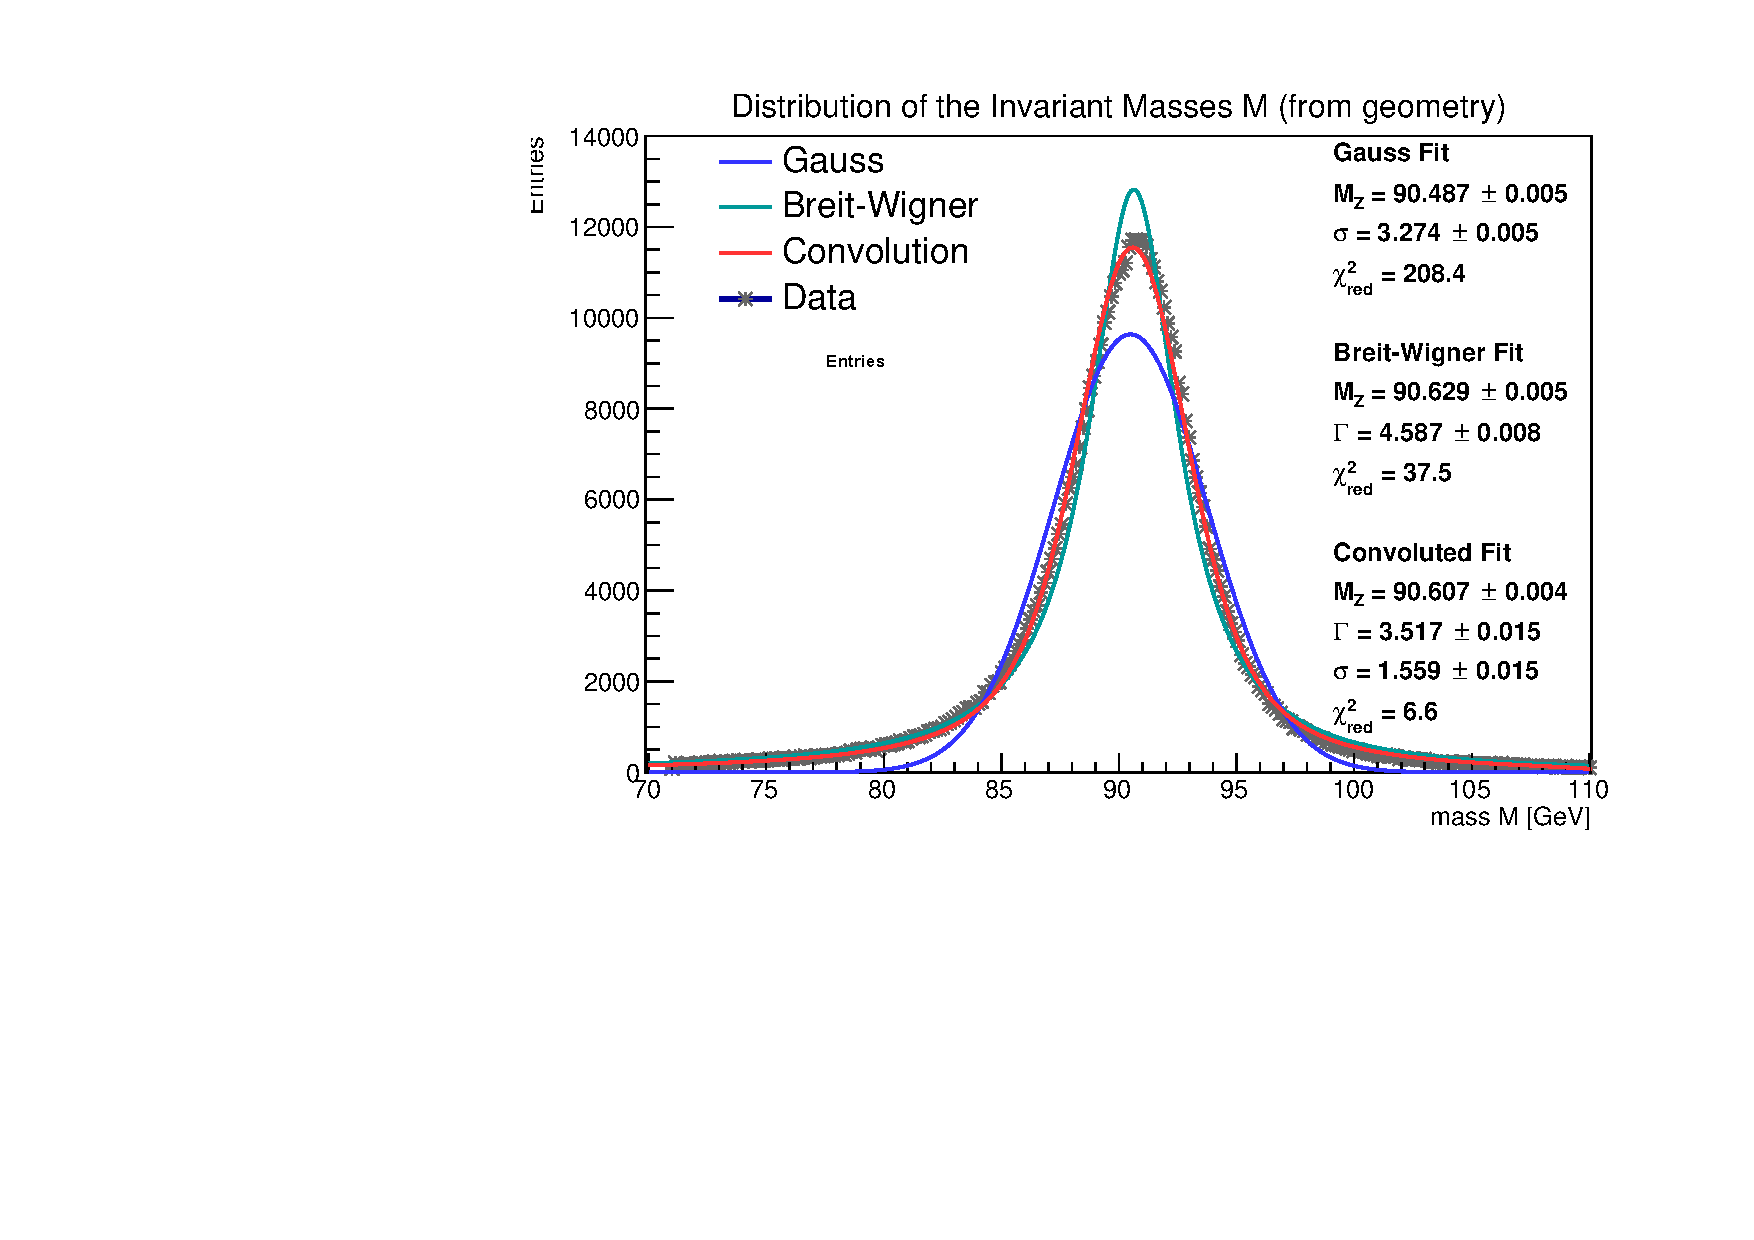
\includegraphics[width = 0.45\textwidth]{figures/plots/ZMassFitted}
	\caption{Distribution of the $Z$ masses $M_z$ with Gaussian, Breit-Wigner and a convoluted fit.}
	\label{fig:MassDist}
\end{figure}

To obtain a satisfying fitting result one needs to convolute a Breit-Wigner distribution and a Gaussian. This is explained by the fact, that the decay process is in theory perfectly described by a Breit-Wigner distribution, but one needs to take the smearing of the curve due to uncertainties in the measure electronics into account which are approximately described by a Gaussian curve. As one can easily see in figure (\ref{fig:MassDist}), the fits using only one of the two functions did not represent the physical model in an adequate manner.
The results from the convoluted fit are presented in the following. \\

For the mass of the $Z$ boson we found
\begin{align}
	M_Z = (90.607 \pm 0.004) \ \text{GeV},
\end{align} 
the decay width $\Gamma$ is
\begin{align}
\Gamma = (3.517 \pm 0.015) \ \text{GeV},	
\end{align}
and the the Gaussian we used to describe the smearing of the distribution due to the measurement process has a standard deviation of 
\begin{align}
	\sigma = (1.559 \pm 0.015) \ \text{GeV}.
\end{align}

\textbf{Theoretical expectations.} \\
Using data from the \href{http://pdg.lbl.gov}{Particle Data Group}, we compare our results to the officially published values. These are 
\begin{align}
	M_{Z,\text{PDG}} = (91.1876 \pm 0.0021) \ \text{GeV},
\end{align} 
and
\begin{align}
	\Gamma_{\text{PDG}} = (2.4952 \pm 0.0023) \ \text{GeV}.
\end{align}

%TODO: Abweicung explizit ausrechnen.. bisschen erkl�ren

\section{Discussion}




\begin{acknowledgments}
We would like to thank our supervisor Philipp Ott for his guidance throughout the operation of this experiment.

\end{acknowledgments}

\bibliographystyle{abbrv}
\bibliography{bibliography/literatur}
\nocite{*}

\end{document}
